\documentclass[11pt]{article}
\usepackage[left=3cm, right=3cm, top=3cm, bottom=3cm]{geometry}
\usepackage[gen]{eurosym}
\usepackage{pdfpages}
\usepackage[utf8]{inputenc}
\usepackage{graphicx}
\usepackage{amssymb}
\usepackage{amsmath}
\graphicspath{ {figures/} }
\usepackage{array}
\usepackage{graphicx}
\graphicspath{ {./verslag_figuren/} }
\begin{document}

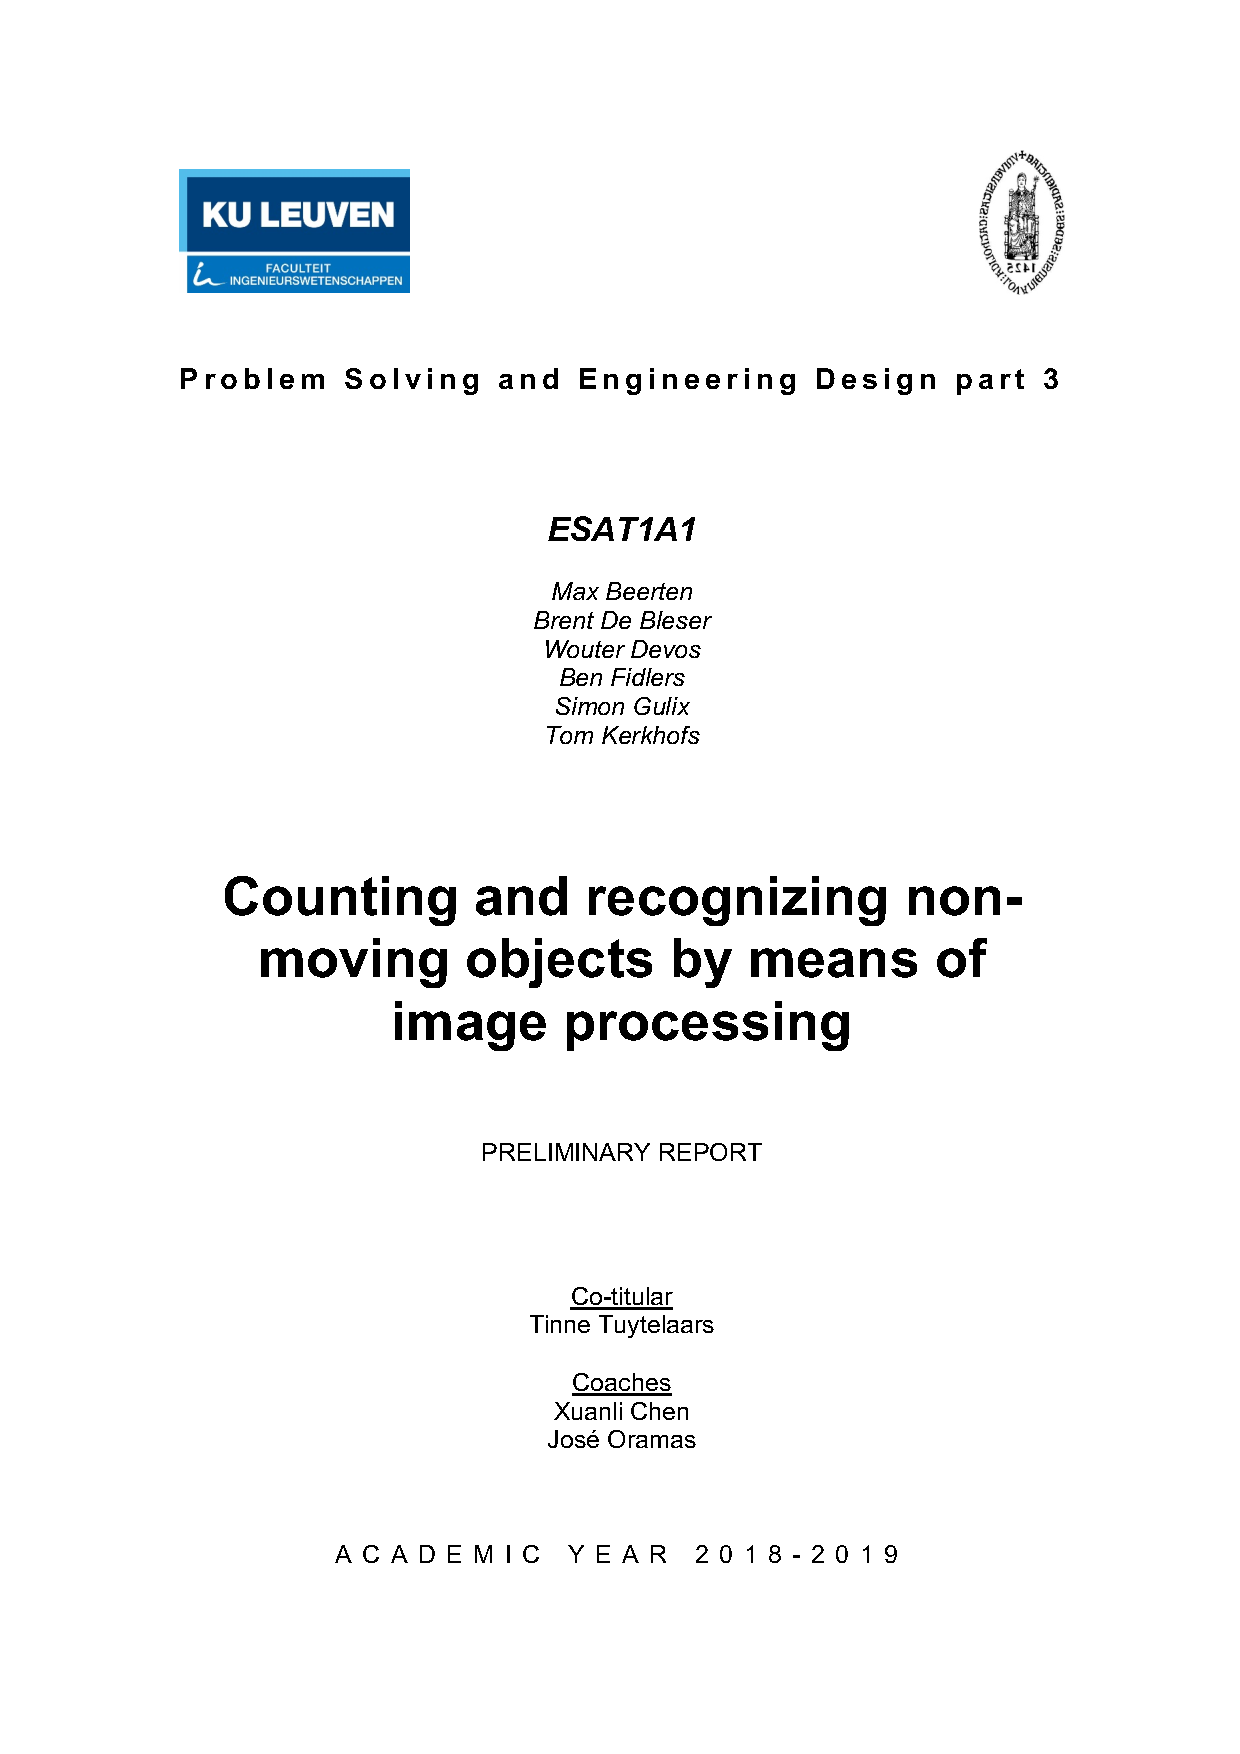
\includepdf[pages=-]{frontpage.pdf}

\section*{Abstract}
\thispagestyle{empty}

\newpage
\tableofcontents
\thispagestyle{empty}

\newpage
\listoftables
\thispagestyle{empty}


\tableofcontents

\section{List of tables and figures}
hier komt een lijst van tabellen, figuren en afkortingen

\newpage
\listoffigures
\thispagestyle{empty}

\newpage
\section{Introduction}
\pagenumbering{arabic}

Digital image processing has been a crucial part of the current digitalisation movement. From industrial machinery to customer amusement, the vision of computer-aided systems has become a given for most users. While image alteration and manipulation remain a core part of this image processing, nowadays other image related problems are being solved by artificial intelligence. Most were considered to be an important part of digital image processing. In this category sits the problem considered in this paper: feature extraction. The counting of objects in an image to be more exact. So why use 'traditional' methods to solve this problem? While being a great way for unravelling many problems, artificial intelligence, mostly provides general solutions. However, certain cases are solved more efficiently by specific methods. Such is the case with object counting, while deep learning algorithms need a big data set as training material, standard image processing only requires the image itself.\\


Regardless which way a method processes images, it needs a visual source. In this paper the focus is on live object counting, which is only possible with a camera. Evidently, the choice of hardware greatly impacts the methods that can be used. This choice will be covered in !TITEL HARDWARE HERE!.\\ 
By far the most important part of this task is the algorithm by which the the objects will be counted. Classically, object counting algorithms have a standard group of steps: filtering, converting to an intensity matrix, edge detection, converting to a binary matrix, boundary boxing and the counting itself. These segments don't have a fixed order and can occur multiple times in the final method. Most of these steps can also be approached in different ways. A wide range of possible filters, kernels, edge detection methods, etc. exist, which all have there benefits and drawbacks.!REFERENTIE BOEK! These choices will be discussed in !TITEL SOFTWARE HERE!.\\
These methods, while being the core of the solution, are fairly simple to implement with the use of libraries or built-in functions. In this paper is opted to give a full implementation of these functions in !TITEL IMPLEMENTATION HERE!. If the functions are deemed to be basic, a simple explanation will be given.


\section{Problem Description}

\hspace{\parindent} Object counting as explained and demonstrated in this report, requires a system which can count objects on a plain background in real time. These objects can vary in shape and colour. Both the colour of the background and the shape and colour of the objects are free from restrictions.\\
The simplest objects, which the system is required to count, are rectangles, cylinders and circles with a uniform colour.

\noindent Given is a basket with a standard rectangular shape with fixed dimensions. The objective is to count every non-moving object in this basket. If possible, the objects can be outlined by the system, as shown in Figure ~\ref{fig:example}. An optional objective is to be able to measure the circumference of the objects in the basket.\\

\noindent The system used should be based on colour and depth images. The used objects don't have the same colour as the basket and/or have a noticeable depth. Otherwise the camera can't notice the objects. the project has to be made with a budget of \euro 250.\\

\begin{figure}[h!]
  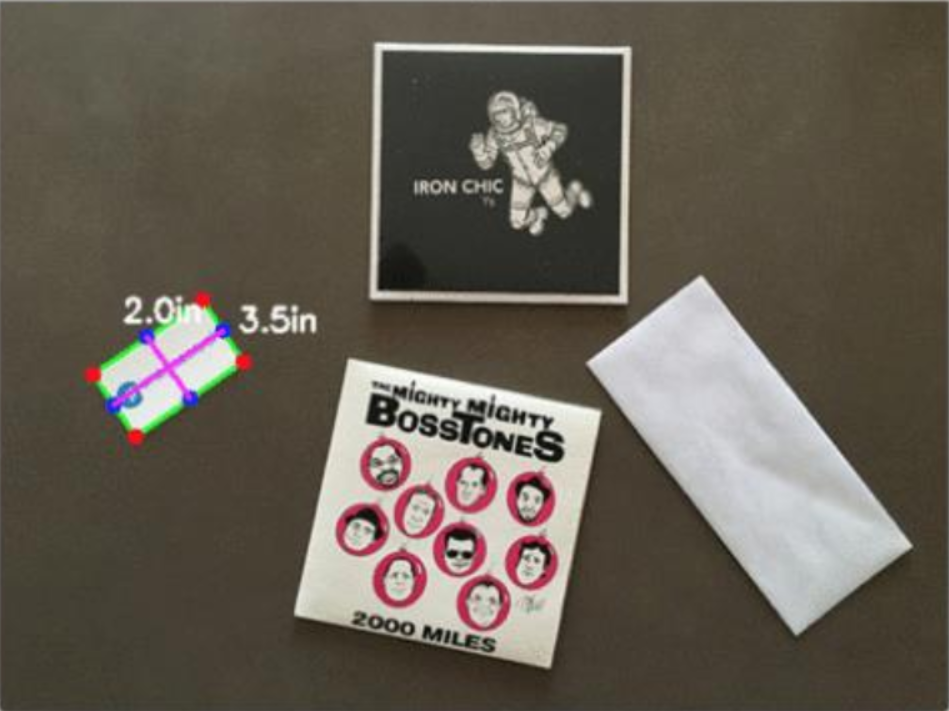
\includegraphics[width=0.7\linewidth]{opdracht.png}
  \caption{The example included in the assignment.}
  \label{fig:example}
\end{figure}



\section{Design}
\subsection{Hardware}
The hardware needed to solve the descripted problem is not complicated. In essence, it just consists of a computer, a camera and a cable to transfer the data between the prior named necissities. Each hardware element is discussed in the following section. \\Choosing the camera is a vital element in this project. If chosen poorly, it can fiercely limit the outcome of the final algorithm. There are three main options in the visual department: a webcam, an industrial camera or a camera with a built-in depth sensor. Each has its pros and cons. A webcam is cheap but doesn't insure good quality and easy acces to its data. A camera for industrial usage is rather expensive. Note that those at the cheaper end of the industrial spectrum only deliver greyscale images. Thirdly, the depth sensing cameras are at a mediocre price point and deliver good quality data. In thought of this specific project the latter is prefered. More specifically is this paper based on a Kinect V2 made by Microsoft. This camera has a color lens with a resolution of 1920 by 1080 and a corresponding field of view of 84.1 by 53.8 degrees. The high resolution ensures an accurate matrix representation of the real image. Each color frame pulled from the Kinect v2 is represented by an array structure of 1080 x 1920 x 3. Every element corresponds with a pixel of the image and varies between 0 and 255. Obviously it can be separated into three different matrices each in $\mathbb{R}^{2}$ and based on a different color of the RGB spectrum. Next to the color camera, the Kinect also possesses a depth sensor. An infrared projector and camera make this possible. It provides a 424 x 512 array making the depth image one of roughly 200 000 pixels. The field of view of this function is 70.6 by 60 degrees. Note that the depth camera provides data about parts of the environment that the color camera does not see, vice versa also. When the computer reads the depth data, every number in the matrix represents a distance in millimeters. Obviously there are some restrictions. This technology only provides correct information if the object is at a distance located in between half a meter and 4 meters. This has to be taken into account for further implementation of this paper.
\\ As second element of hardware has the computer a less important role. Preferably, OSX isn't used as operating sytem for this application because the Kinect drivers don't exist for Macintosh computers. If the reader has a Mac, problems can be avoided by running Windows/Ubuntu via a virtual machine. Speed of the used computer system isn't anything to worry about. The algorithm should run in an acceptable timeframe on every machine.\\ To conclude this section a brief word on the necessary transfer cable. Since a depth sensing camera is used, two types of data (depth and color) need to be transfered. The Microsoft OEM Kinect Adapter makes this possible. The special adapter consists of two general parts . One part in function of delivering current to the camera and the other to transfer both types of data to the connected computer. 

\subsection{Software}
\subsubsection{Analysis colour image }
There are a lot of options when it comes to software and a wide range of different algorithms exist for image processing. The diagram on FIG…XX… shows a couple of different methods. There is no ‘right-way’ to count objects in an image. Different approaches have their own advantages and disadvantages. The only things that are common for most algorithms are:
\begin{itemize}
\item Converting the RGB image to grayscale
\item Run filters over the image to remove noise
\end{itemize}
These elements are also visible in the diagram.
\paragraph{Method 1}\mbox{}\\
This method is the most simple and easy to implement. As input, it takes a filtered greyscale image. This is run trough a thresholding-algorithm with a pre-defined threshold value. The output is a binary matrix. This array only has 0's and 1's, respectively representing the colours white and black. The key to solving the problem in this way is writing code that finds the treshold value based on environmental parameters. When in posession of a real black and white image, a simple edge detection program is run which makes the edges visible. 
\\Advantages: It’s an easy and fast algorithm.
\\Disadvantages: With a pre-defined threshold value it just classifies pixels based on colour. 
\paragraph{Method 2}\mbox{}\\
Method 2 tackles the colour analysis in the opposite order than method 1, as it starts with an edge detection algorithm. Since the input image is still very complex, this edge detection is way more comprehensive. The output is a greyscale image, contrary to the binary array the reader might expected. This is followed by some tresholding code with a pre-defined treshold value. The current image is now represented by a matrix where the edges are represented in binary. Viewing the fact that there is a lot of noise using this sequence of steps, it's recommended to include noise reduction code. 
\\Advantages: It detects all kind of objects, not based on colour or shape.
\\Disadvantages: The boundary between different objects needs to be clear for this to work.
\paragraph{Method 3}\mbox{}\\
<<<<<<< HEAD
The third way takes a different approach to solving the analysis of the colour image. When using this, a compromise in functionality is made. Since it needs a picture of the empty background without any objects, the user experience is worsened. After getting a background image, the picture of the situation with objects gets filtered and the algorithm converts it into a greyscale image. Using this less complex matrix, the code loops through the image pixel by pixel. This necessary but time consuming loop checks if the pixel on the image is more or less the same as the corresponding pixel on the background image. If located within a pre-determined range, that element of the array gets classified as background. The consequence is that the output is a binary image with clear-cut objects.
Advantages: It is very good in detecting objects, not being based on colour or shape.
Disadvantages: There needs to be an image of the empty background. Note that the lighting conditions have to be unaffected in between taking the needed pictures for this algorithm.


The third way takes a different approach to solving the analysis of the colour image. When using this, a compromise in functionality is made. Since it needs a picture of the empty background without any objects, the user experience is worsened. After getting a background image, the picture of the situation with objects gets filtered and the algorithm converts it into a grayscale image. Using this less complex matrix, the code loops through the image pixel by pixel. This necessary but time consuming loop checks if the pixel on the image is more or less the same as the corresponding pixel on the background image. If located within a pre-determined range, that element of the array gets classified as background. The consequence is that the output is a binary image with clear-cut objects.
\\Advantages: It is very good in detecting objects, not being based on colour or shape.
\\Disadvantages: There needs to be an image of the empty background. Note that the lighting conditions have to be unaffected inbetween taking the needed pictures for this algorithm.

\paragraph{Implementation}\mbox{}\\
\begin{figure}[h]
\caption{Example of a parametric plot ($\sin (x), \cos(x), x$)}
\centering
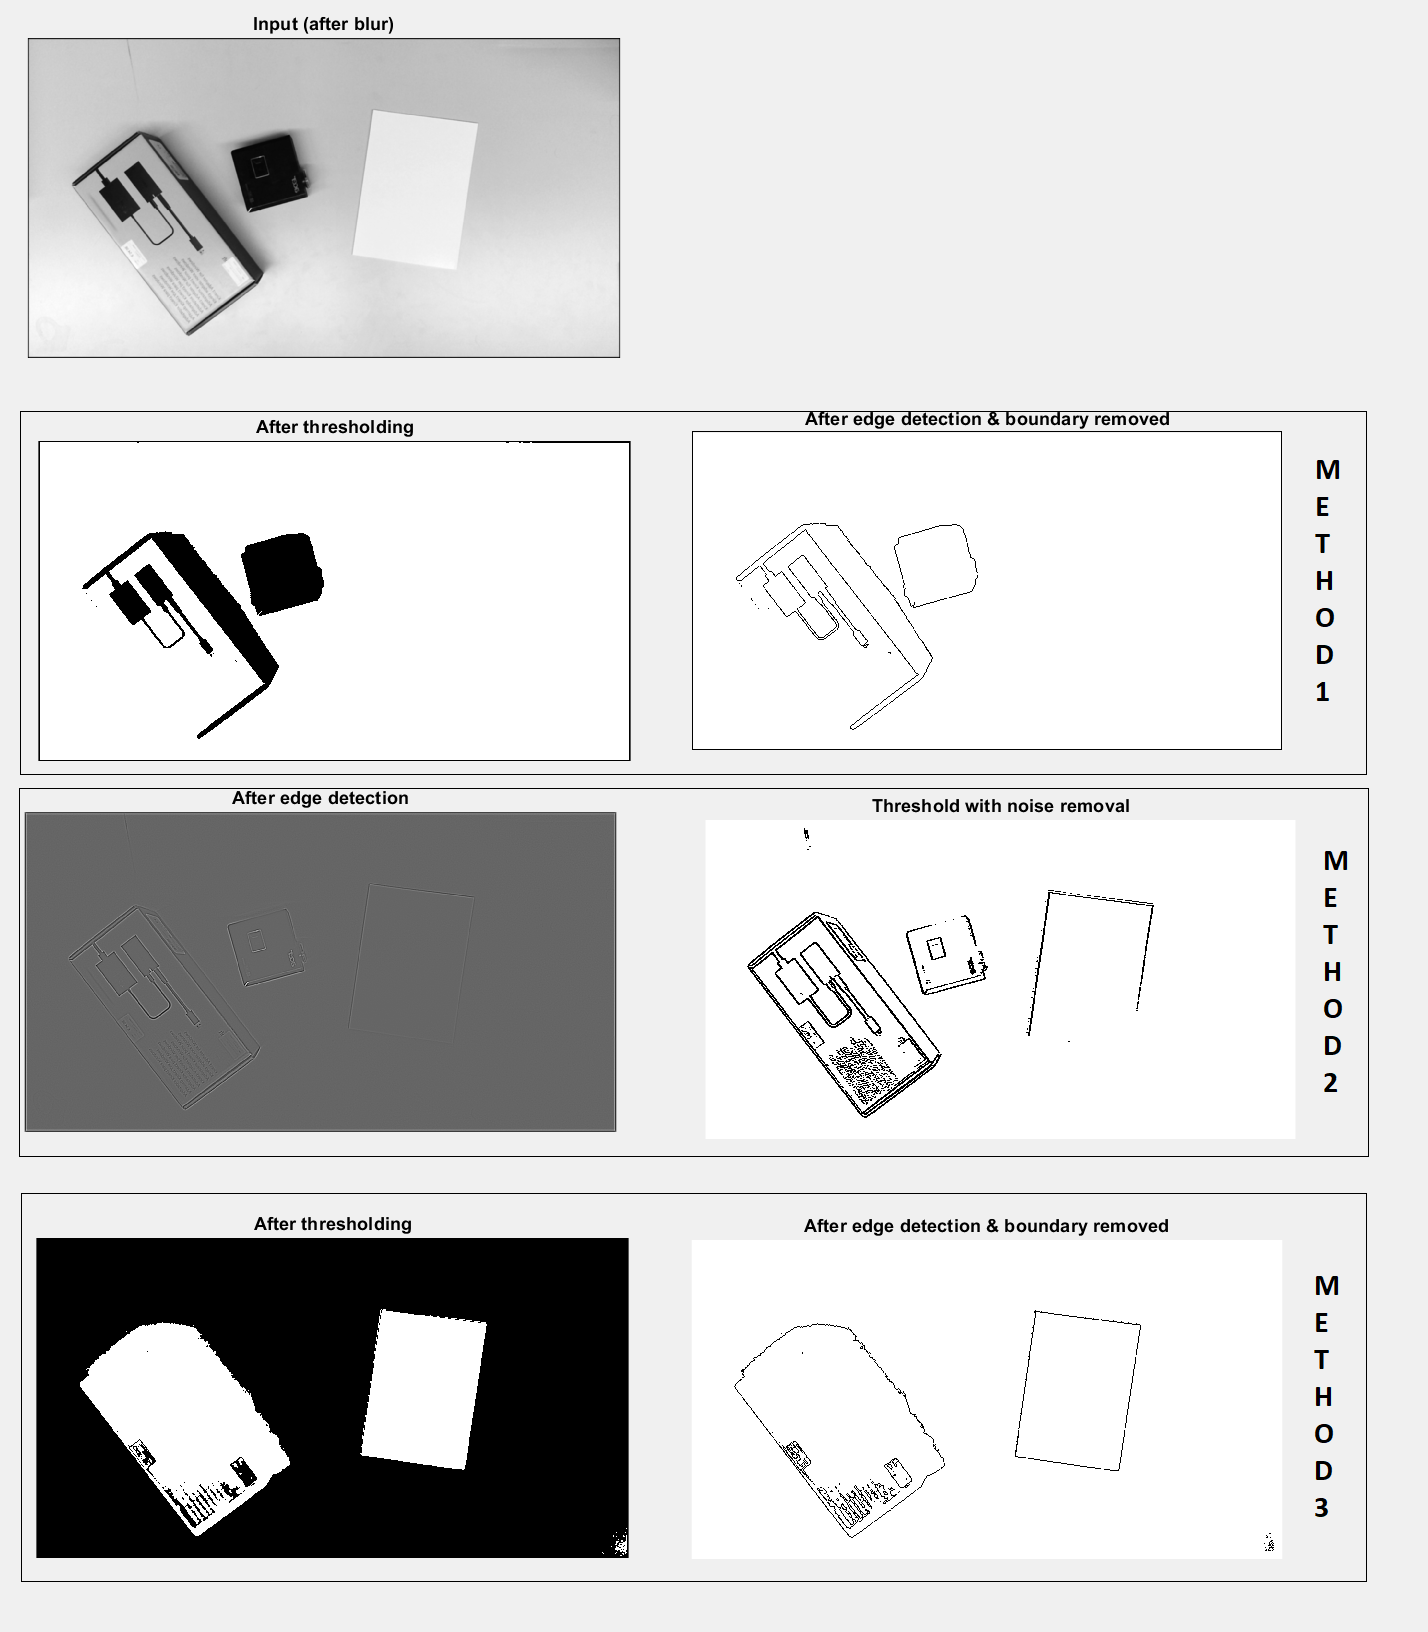
\includegraphics[width=0.5\textwidth]{comparison_methods}
\label{fig:comparison_methods}
\end{figure}

After a lot of testing different methods, the three methods above seemed the most interesting. After comparing these methods with each other, it seems that method 2 is the best choice. See figure \ref{fig:comparison_methods} for the comparison. As mentioned above, the fist thing that needs to be done with the image is converting it to grayscale. An RGB image exists from colors: red, green and blue. Thus an RGB image is a 3-dimensional matrix. The grayscale image is calculated by multiplying the individual color values with a color-specific weight. So loop through every pixel and combine the 3-dimensional RGB matrix to a 1-dimensional grayscale image.
\begin{equation}
grayscale\_image(row, col) = 0.2989 * RED + 0.5870 * GREEN + 0.1140 * BLUE
\end{equation}
All the weights count up to 1 so the values in the grayscale image can vary from 0 to 255.
\\This method uses two filters to remove noise from the image. Figure XXXX shows why those two filters are necessary.
At first the gaussian blur, this is an easy convolution on the image matrix.
\begin{equation}
  G = (1/159) * 
  \begin{bmatrix}
   2 & 4 & 5 & 4 & 2\\
   4 & 9 & 12 & 9 & 4\\
   5 & 12 & 15 & 12 & 5\\
   4 & 9 & 12 & 9& 4\\
   2 & 4 & 5 & 4 & 2
  \end{bmatrix}
\end{equation}
The blur can be applied by doing a convolution of the G matrix on the image matrix.
The second blur is a mean blur. This is another matrix to do the convolution with.
\begin{equation}
M = (1/9) * 
\begin{bmatrix}
	1&1&1\\
	1&1&1\\
	1&1&1
\end{bmatrix}
\end{equation}
Then comes the edge detection algorithm, this basically just a filter. So it is possible to calculate another convolution. It calculates the \textit{spatial  derivative}, this refers to how much the image intensity values change per change in image position. It highlights regions of rapid intensity change.
\begin{equation}
L =\begin{bmatrix}
	0&-1&0\\
	-1&4&-1\\
	0&-1&0
\end{bmatrix}
\end{equation}
A convolution with this returns a matrix the same size as the input image matrix, but the values can now be negative. More negative is darker. The threshold algorithm is based off this feature. After a lot of experimenting it seemed that a threshold of value 2 was the sweet spot. This means that every pixel greater than or equal to that threshold value becomes an edge, and the rest gets classified as background. After applying that algorithm, the image becomes a binary image with only the edges in black. Finding the edge of an object is one thing, couting objects is another. Based of these edges it's possible to outline the objects and count them. Further programming has to be done to reach our goal and complete this algorithm.


\subsubsection{Depth sensor}
\subsubsection{Analysis Depth Sensor}
Using only the RGB image does have some shortcomings: it is rather difficult to distinguish an object from its shadow, a multicoloured object could be seen as multiple different objects or a lot of reflection could make an object undetectable. These are some of the reasons why enrichening the object counting algorithm with the usage of a depth sensor is advised. The data enters the system in a matrix in which every number stands for the distance between the sensor and the object (in millimeters). Firstly the code should be able to see a clear difference in height between the objects and the background. After that the noise that can exist will be filtered out. At last the cleaned matrix will be used to detect the edges of the objects and thus detect the objects themselves.
 
\paragraph{Detection of the difference in height}\mbox{}\\
At first, the goal is to see a clear difference between the objects and the background. This can be achieved in different ways: it is possible to use a treshold and call everything closer than a predetermined value an object. A disadvantage of this method is that this value will be different for different positions of the sensor. Also, the image of the sensor contains some noise. For example, a big surface with every point at the same height will not return a matrix filled with the same number at every location. Another, and more preferred, method would be to use a Sobel-Feldman operator \textbf{[hier komt verwijzing naar boek in bronvermelding]}. This operation approximates the gradient in each of the points of the matrix, and so gives an idea where there is a sudden difference in height (thus where there might be an object). It works by convolving 2 kernels with the image matrix A to become $G_{x}$ and $G_{y}$ respectively one for the horizontal and one for the vertical change in height. The overall gradient is equal to 
\paragraph{filtering of the noise}\mbox{}\\

\paragraph{Edge detection of the objects}\mbox{}\\

\section{Implementation}
Throughout the project a lot of different approaches were tested and discarded. But in essence they all do the same thing they convert the original image to a binary image. In this binary image the objects are represented by one value and the background by another. Afterwards this binary image is analysed and a simple algorithm suffices to count the objects. In this fase of the program the same code is applicable. This code consists of a few important parts: the actual counting and the drawing of the boundary boxes. 

Throughout the project a lot of different approaches were tested and discarded. But in essence ,they all do the same thing. They convert the original image to a binary image. Afterwards, this binary array is analysed and a simple algorithm suffices to count the objects. In this fase of the program the same code is applicable. This code consists of a few important parts: the actual counting and the drawing of the boundary boxes. 
\paragraph{Counting of the objects}\mbox{}\\
The central objective of this paper is counting the amount of objects in a specific rectangular field of view. The general approach to this problem is converting the image to a binary image where black pixels represent the background and white pixels represent the objects. By counting the groups of pixels it is possible to know how many objects the original image contains. In the image processing toolbox for matlab there exist a few functions that come in really handy for this kind of tasks. One of these functions bwlabel actually counts group of pixels of at least 8 that are connected. The syntax of this function goes as follows: [L, num] = bwlabel(BW); where BW represents the binary (or black and white) image; num represents the number of objects in the BW image and where L represents a matrix were the first group of pixels are numbered 1, the second group 2 etc. that way it's easier to get a count for how many objects there are.

\paragraph{Boundary boxes}\mbox{}\\
The image processing toolbox really simplifies the drawing of boundary boxes. Once a binary image is obtained the function regionprops can extract properties about image regions. Where image regions are defined as 8-connected components in an binary image. This means that each image region contains at least 8 interconnected white pixels, since the black pixels are registered as background. The property that's interesting for this part of the project is called 'boundingbox'. This property returns for every image region the smallest rectangle containing this region. In two dimensions this is a vector with 4 values, the x-coordinate of the upper left corner, the y-coordinate of that corner, the width and the height. The function rectangle('Position', pos), where 'Position' declares the input and where pos is the input obtained from regionprops, can easily display this boundingbox. 

\paragraph{Edge detection}\mbox{}\\
Test 123

\section{Steps of implementation}

\subsubsection{Stages of difficulty}

\subsubsection{Previous implementations}

\section{Budget management}

\section{Course Integration}

\section{Conclusion}

\section{List of references}

\section{Appendix}

\end{document}
